% DOCUMENT HEADER
\documentclass{article}
\usepackage[utf8]{inputenc}
\usepackage{graphicx}
\usepackage{pgfplots}
\usepackage{amsfonts}
\usepackage{fancyhdr}
\usepackage{tabularx}
\usepackage{gensymb}
\usepackage{amsmath}
\usepackage{hyperref}

% Set up hyperlinks
\hypersetup{colorlinks=true,
            linkcolor=blue,
            urlcolor=blue}


% TITLE
\title{\textbf{Understanding the Tangent Function}}
\author{\textit{Michal Špano}}
\date{}

% Set up default path for pictures 
\graphicspath{{assets/}}

% Page header
\pagestyle{fancy}
\fancyhf{}
\rhead{MAT, @michalspano}
\lhead{Tangent function}
\rfoot{Page \thepage}

\begin{document}

\maketitle

% SECTION 1
\section{Definition}
To define the $tangent$ function, one must understand the basic principles of deriving $sine$ and $cosine$ using a so-called \textbf{unit circle}.

A \textbf{unit circle} is the circle of radius 1 centred at the origin $O(0, 0)$ in the \textbf{Cartesian coordinate system}.

% Include a picture of a unit circle
\begin{figure}[htp]
    \centering
    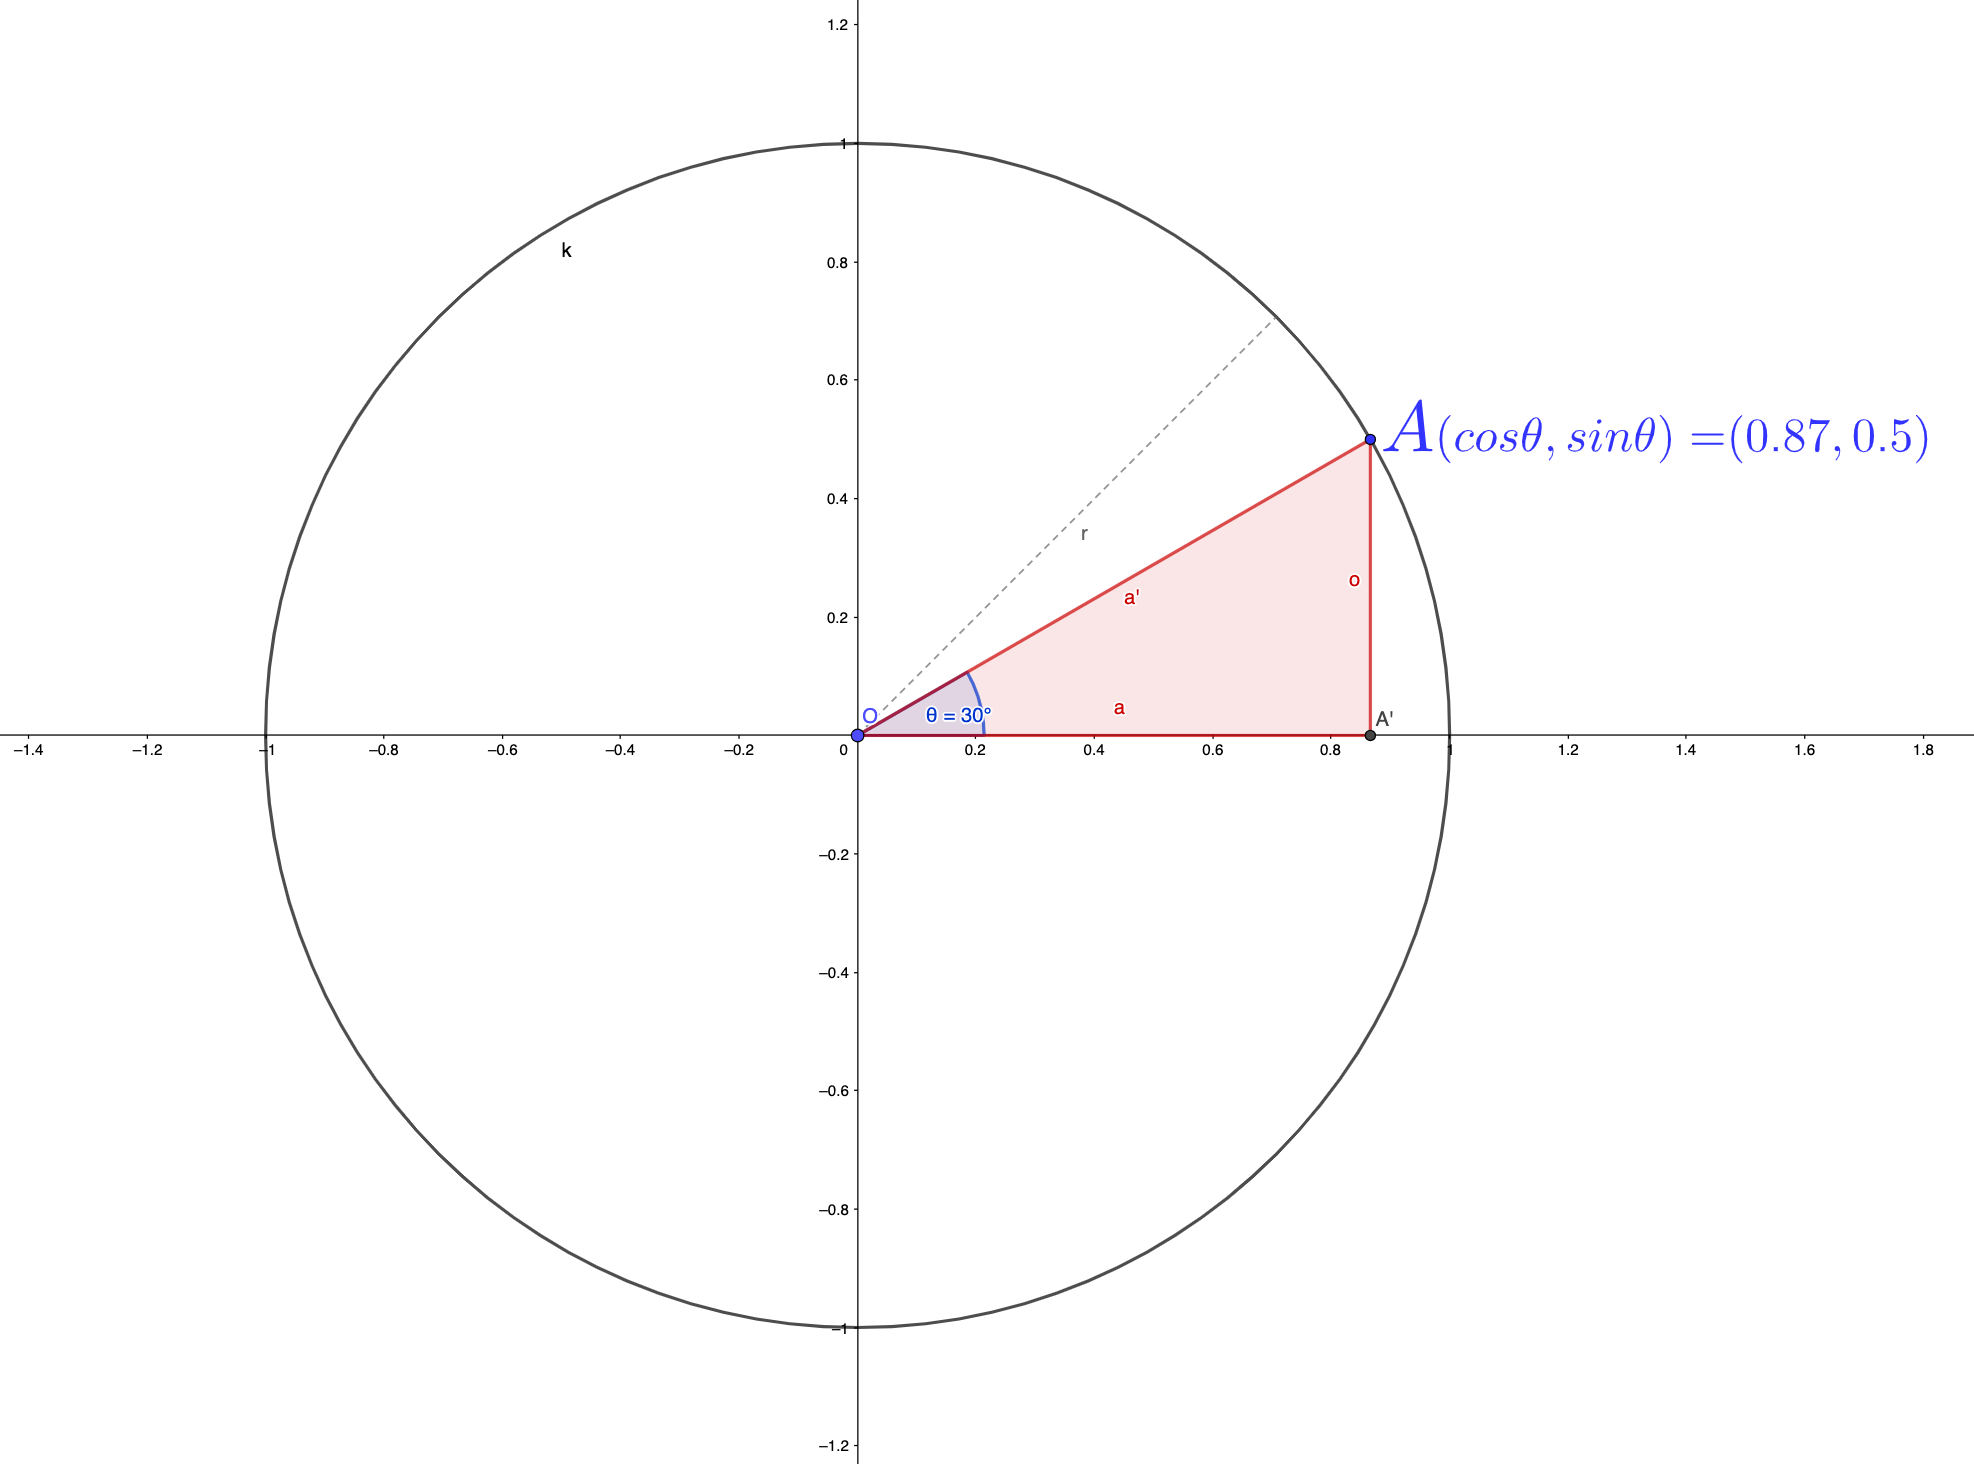
\includegraphics[width=9cm]{unit_circle.png}
    \caption{Unit circle}
\end{figure}

Then for a point $A = [x, y]$ moved along the circumference $k$ by an angle $\theta$ is valid:\\ 
\[  
A = \left[ cos(\theta), sin(\theta) \right]
\]

\textit{Note: an applet is available (\href{https://www.geogebra.org/m/gvtvjtpf}{link}) or scan its \textbf{QR code} under \textbf{Resources}}.

A right-angled triangle consists of the \textbf{hypotenuse} (the side opposing the right angle) and 2 other adjacent sides called \textbf{legs}. The definition of tangent states that it is the quotient of the opposite side and the adjacent side to a certain angle $\theta$, symbolically: 
\[
tan(\theta) = \frac{opposite}{adjacent}
\]

Which can be further transformed into: 
\[
tan(\theta) = \frac{y}{x} ... tan(\theta) = \frac{sin(\theta)}{cos(\theta)}
\]

% SECTION 2
\section{Properties}

Now, let's address the properties of $f:y=tan(x)$

\textbf{Graph: }

% GENERAL GRAPH
\begin{figure}[htp]
    \centering
    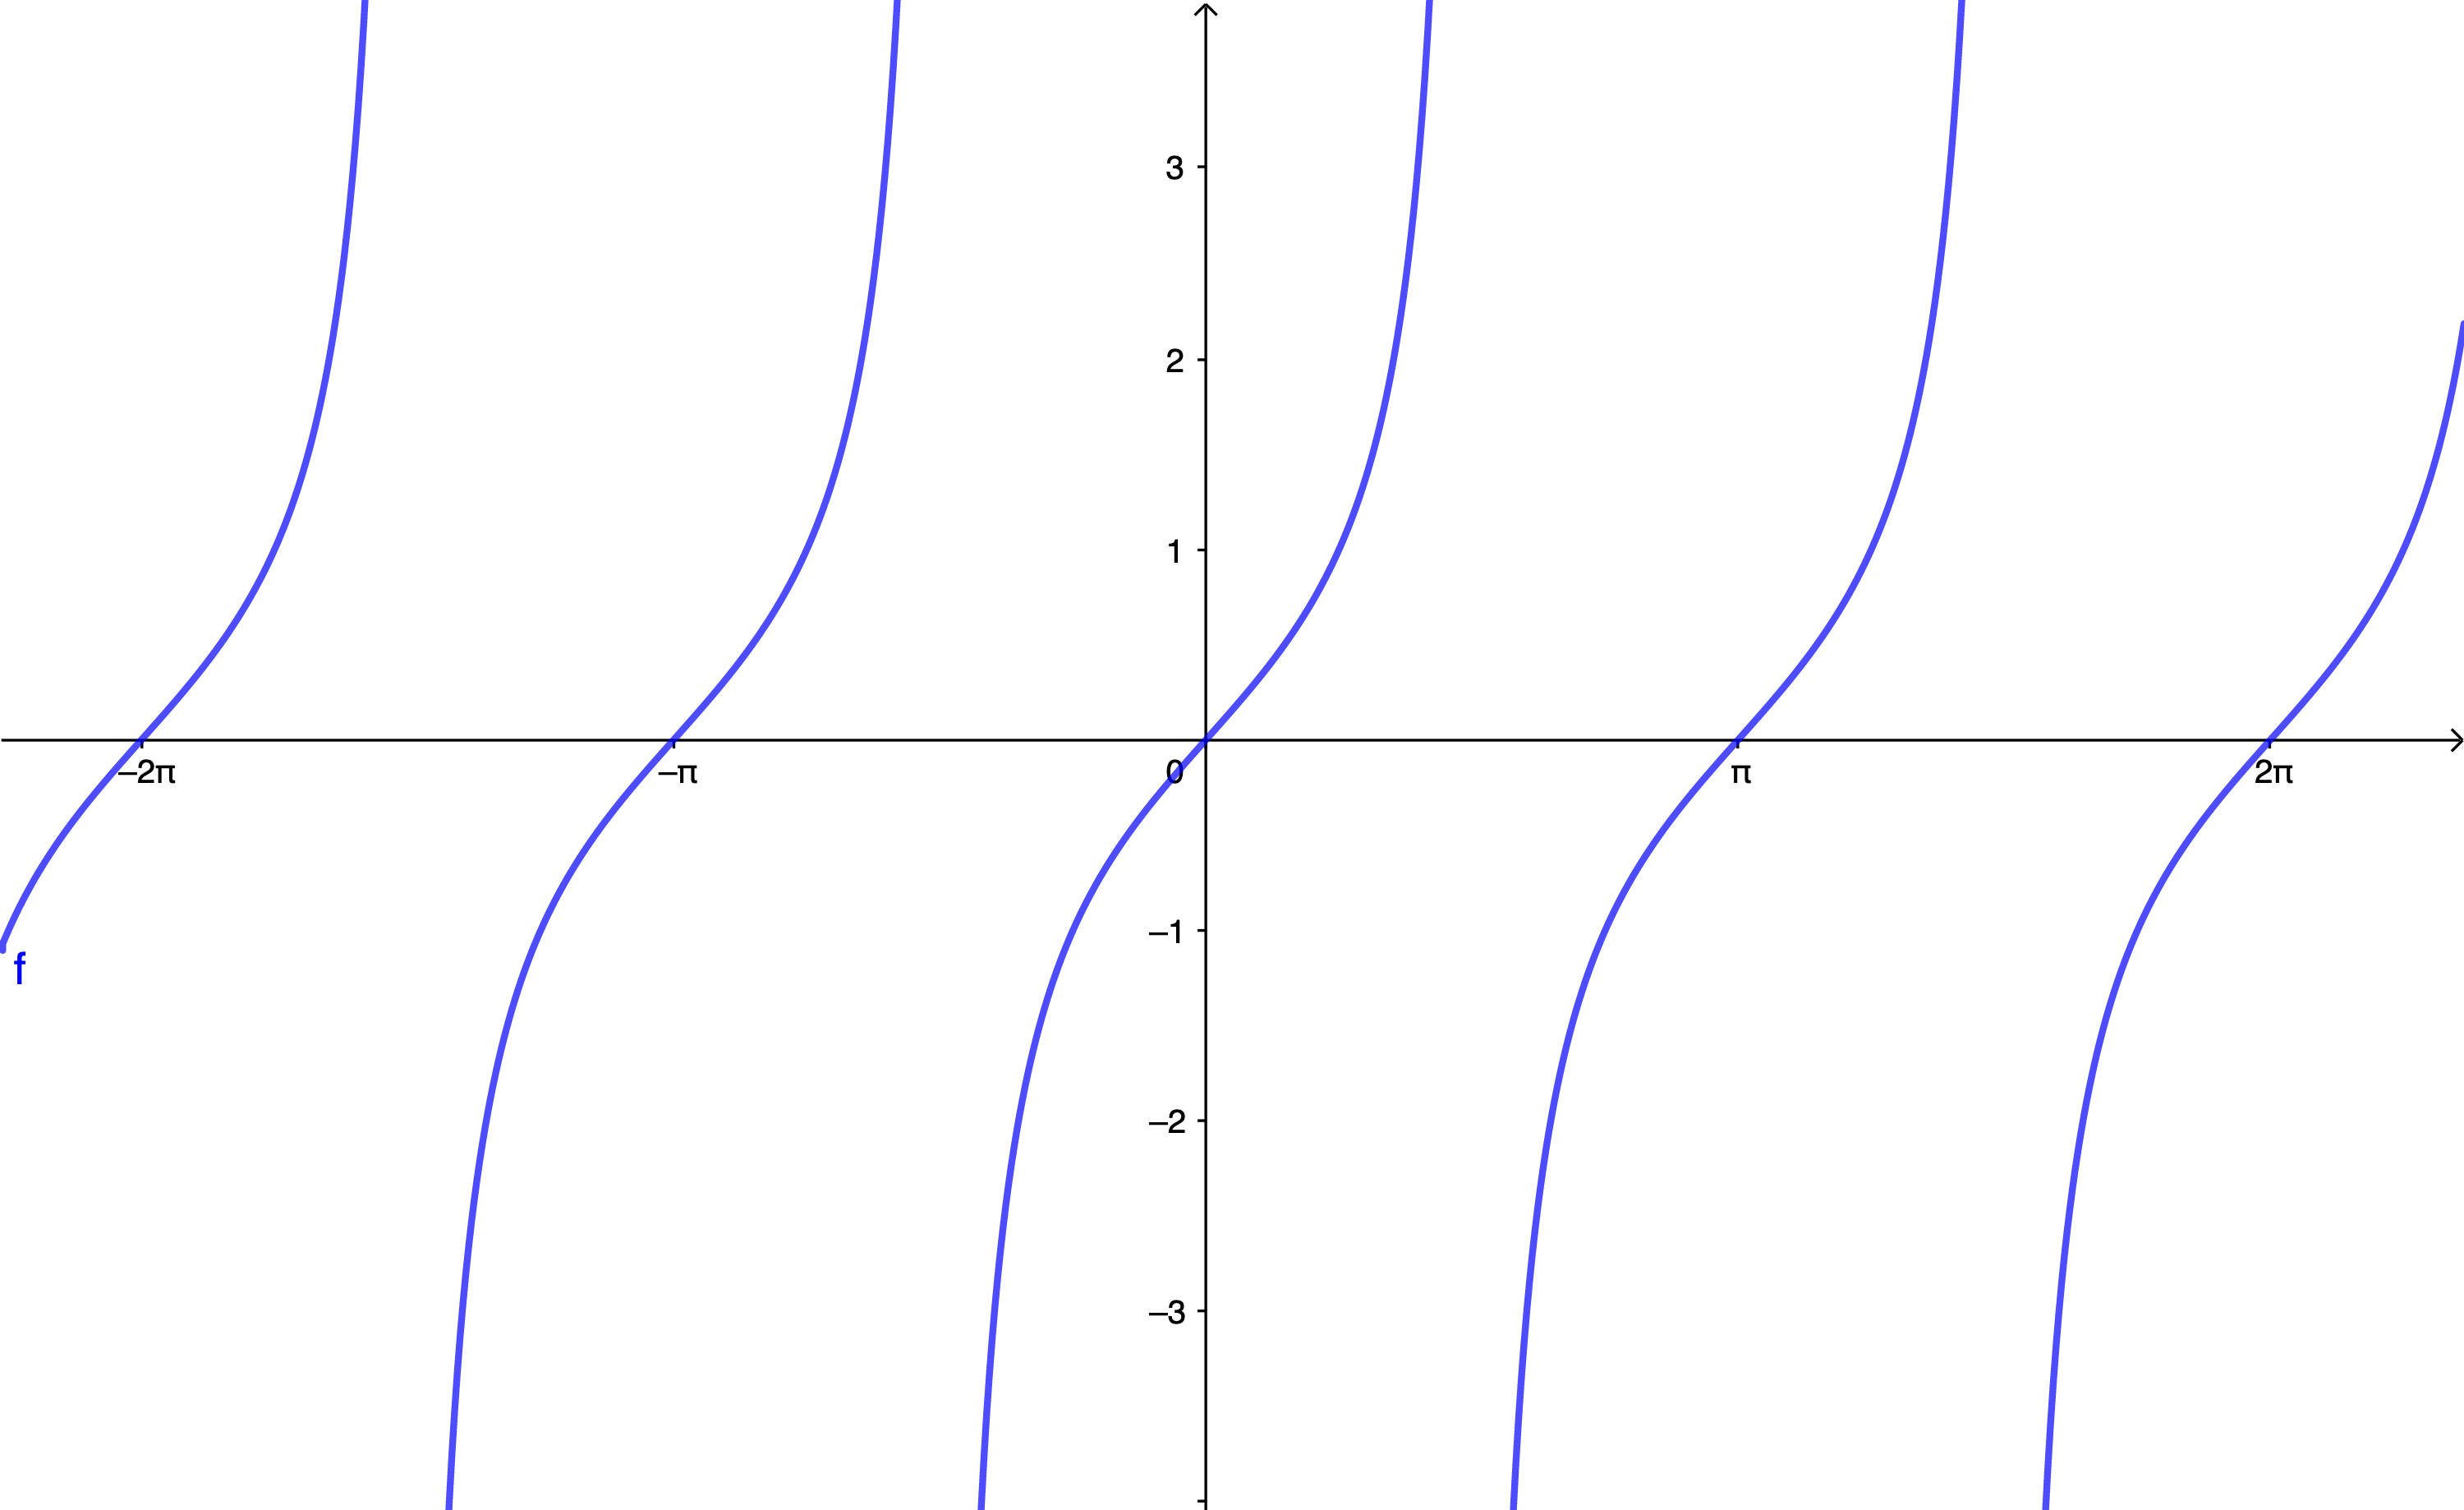
\includegraphics[width=8cm]{tan.png}
    \caption{$y=tan(x)$}
\end{figure}

% ENUMERATED PROPERTIES
% http://www.nabla.hr/TF-TrigFunctionsD3.htm
\textbf{Properties: }
\begin{enumerate}

    % DOMAIN
    \item \textbf{Domain}
    \[
    f:y=tan(x) ... y=\frac{sin(x)}{cos(x)} \Leftrightarrow cos(x) \neq 0
    \]
    
    \begin{figure}[htp]
        \centering
        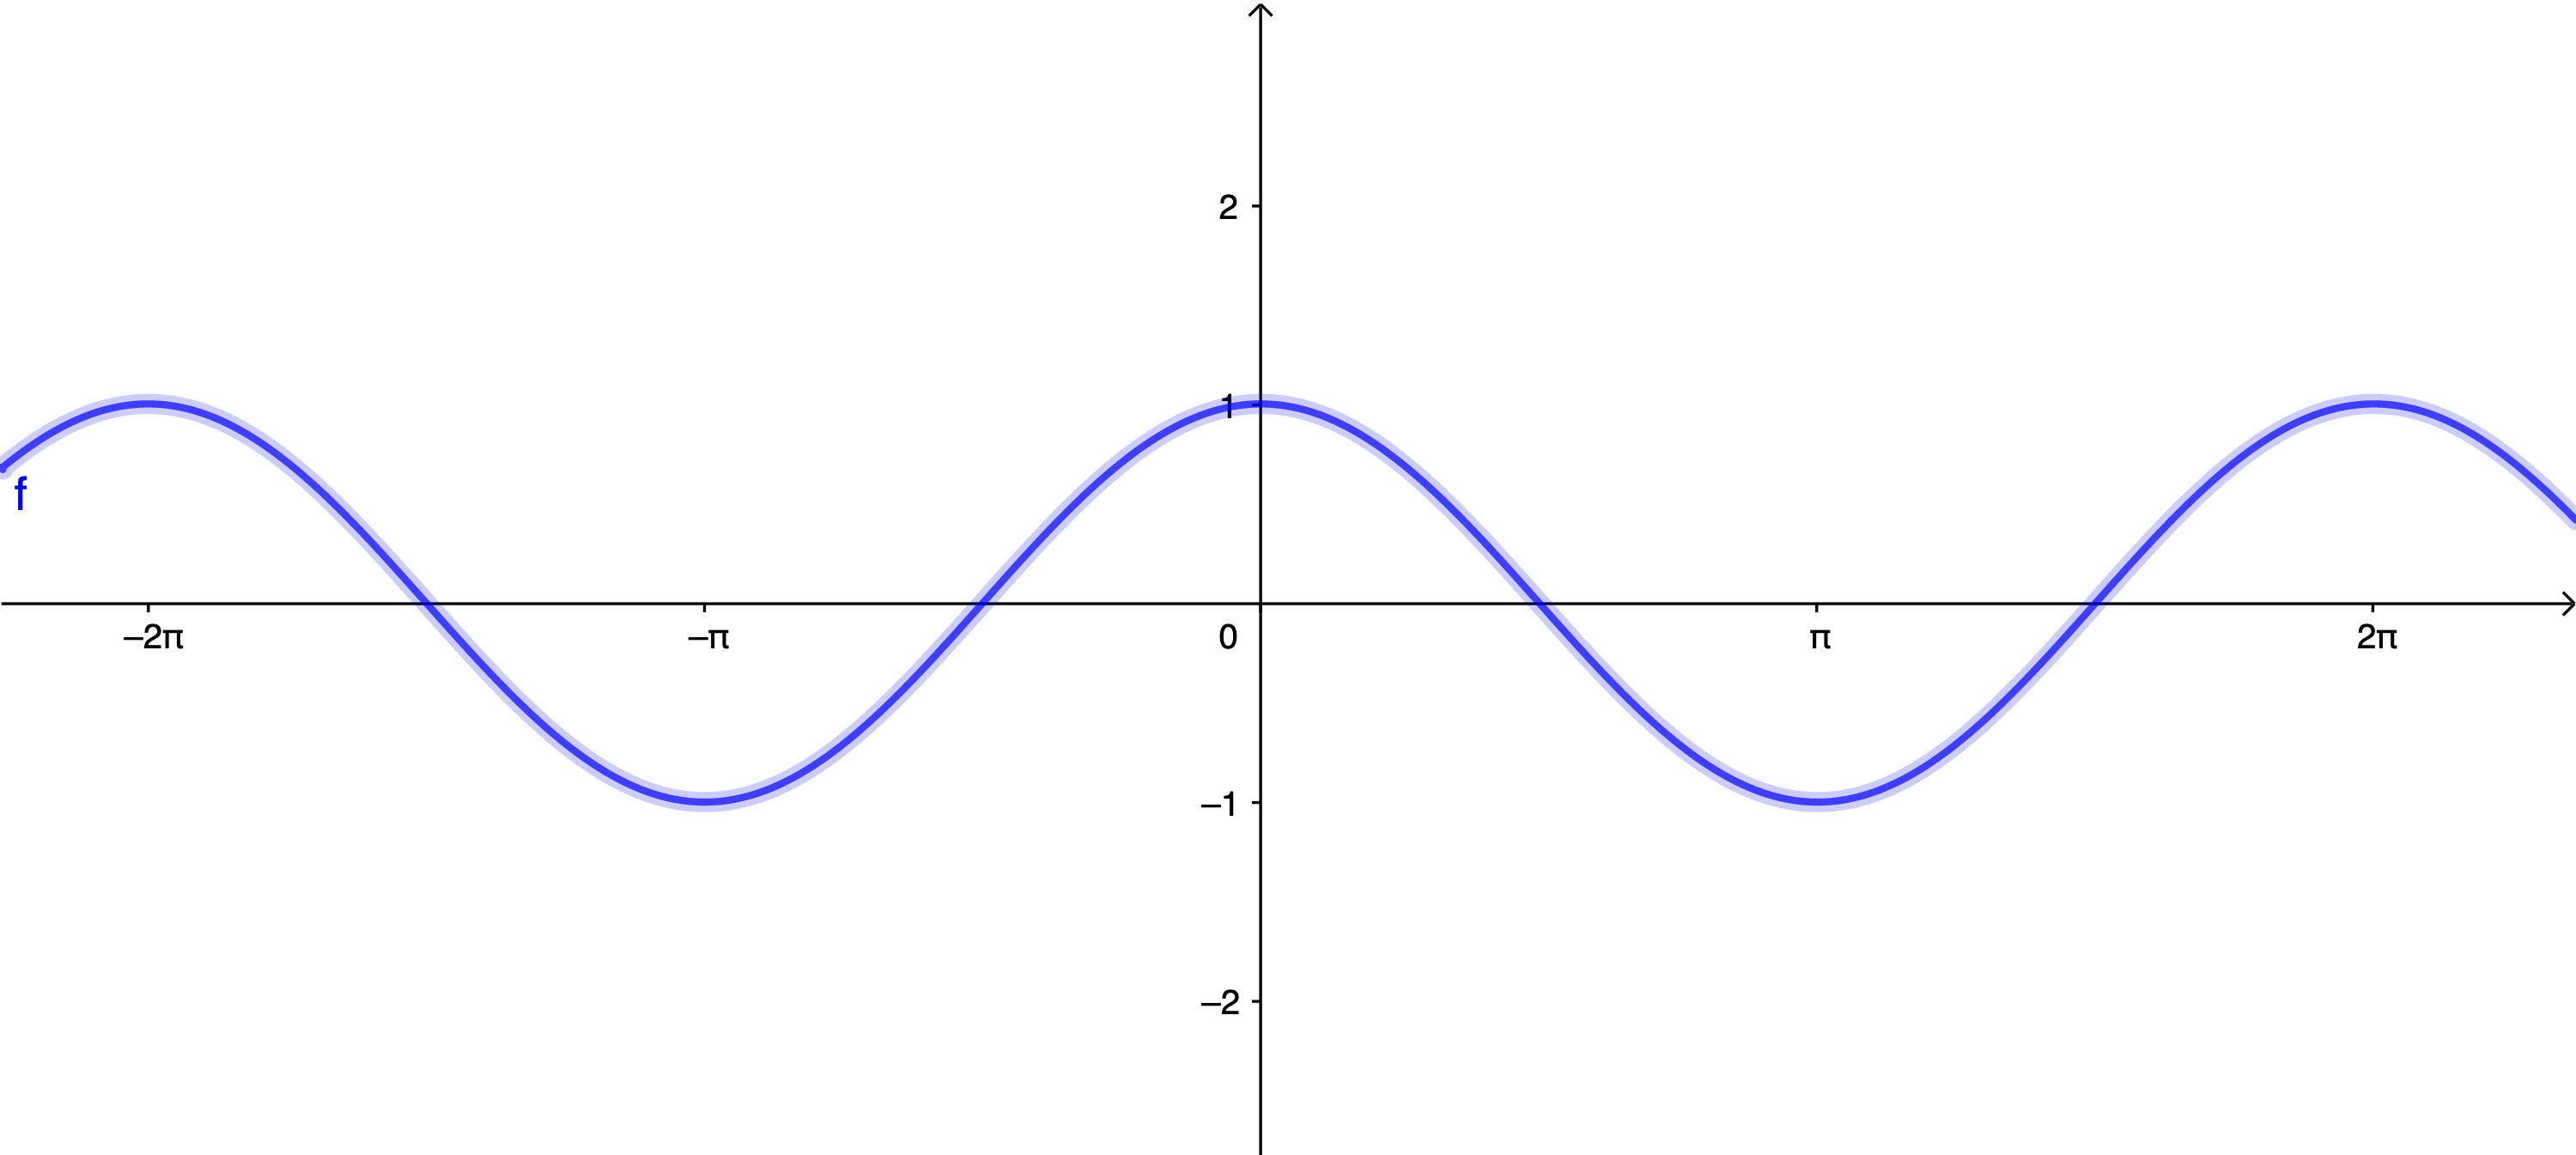
\includegraphics[width=10cm]{cosine.png}
        \caption{$y=cos(x)$}
    \end{figure}    
    
    \textit{Let $f:y=cos(x)$}, solve for $x\in\mathbb{R}$.
    \[
    x \in \Big\{ \frac{\pi}{2}; \frac{3\pi}{2} + 2k\pi, k \in\mathbb{Z} \Big\} \Leftrightarrow
    x \in \Big\{ \frac{\pi}{2} + k\pi, k \in\mathbb{Z} \Big\}
    \]
    Through additional steps, we obtain the following result:
    \[
    x\in\{(2k+1)\frac{\pi}{2}, k\in\mathbb{Z} \}
    \]
    
    In other words, the \textbf{Domain} of $y=tan(x)$ is all real numbers except every $x$ for which is $cos(x) = 0$ defined. Symbolically:
    \[
    D_f= \mathbb{R}-\{ (2k+1)\frac{\pi}{2}, k\in\mathbb{Z} \}
    \]
    
    % Range of values
    \item \textbf{Range of values}
    
    As shown in the figure above, the \textbf{Range} of $f: y=tan(x)$:
    \[
    H_f=\mathbb{R}
    \]
    
    % Values in quadrants
    \item \textbf{Values in quadrants}
    
    \begin{center}
    \begin{tabular}{||c c c c||} 
    \hline
    \textit{I.} & \textit{II.} & \textit{III} & \textit{IV} \\ [0.5ex] 
    \hline\hline
    $\Big(0;\frac{\pi}{2}\Big)$ & $\Big(\frac{\pi}{2};\pi\Big)$ & $\Big(\pi;\frac{3\pi}{2}\Big)$ & 
    $\Big(\frac{3\pi}{2};2\pi\Big)$ \\
    \hline
    + & - & + & - \\ [1ex] 
    \hline
    \end{tabular}
    \end{center}
    
    % Periodicity of tangent
    \item \textbf{Periodicity}
    
    Suppose that the $period$ of $y=tan(x)$ is $2\pi$: 
    \[
    tan(x + 2k\pi) = \frac{sin(x + 2k\pi)}{cos(x + 2k\pi)} = \frac{sin(x)}{cos(x)} = tan(x)
    \]
    However, $2\pi$ is not the smallest possible period. Let us consider a case where $period$ is $\pi$.
    \[
    tan(x + \pi) = \frac{sin(x +\pi)}{cos(x + \pi)} = \frac{-sin(x)}{-cos(x)} = tan(x)
    \]
    
    % Include graphical depiction
    \begin{figure}[ht!]
        \centering
        \vspace{-10pt}
        \centering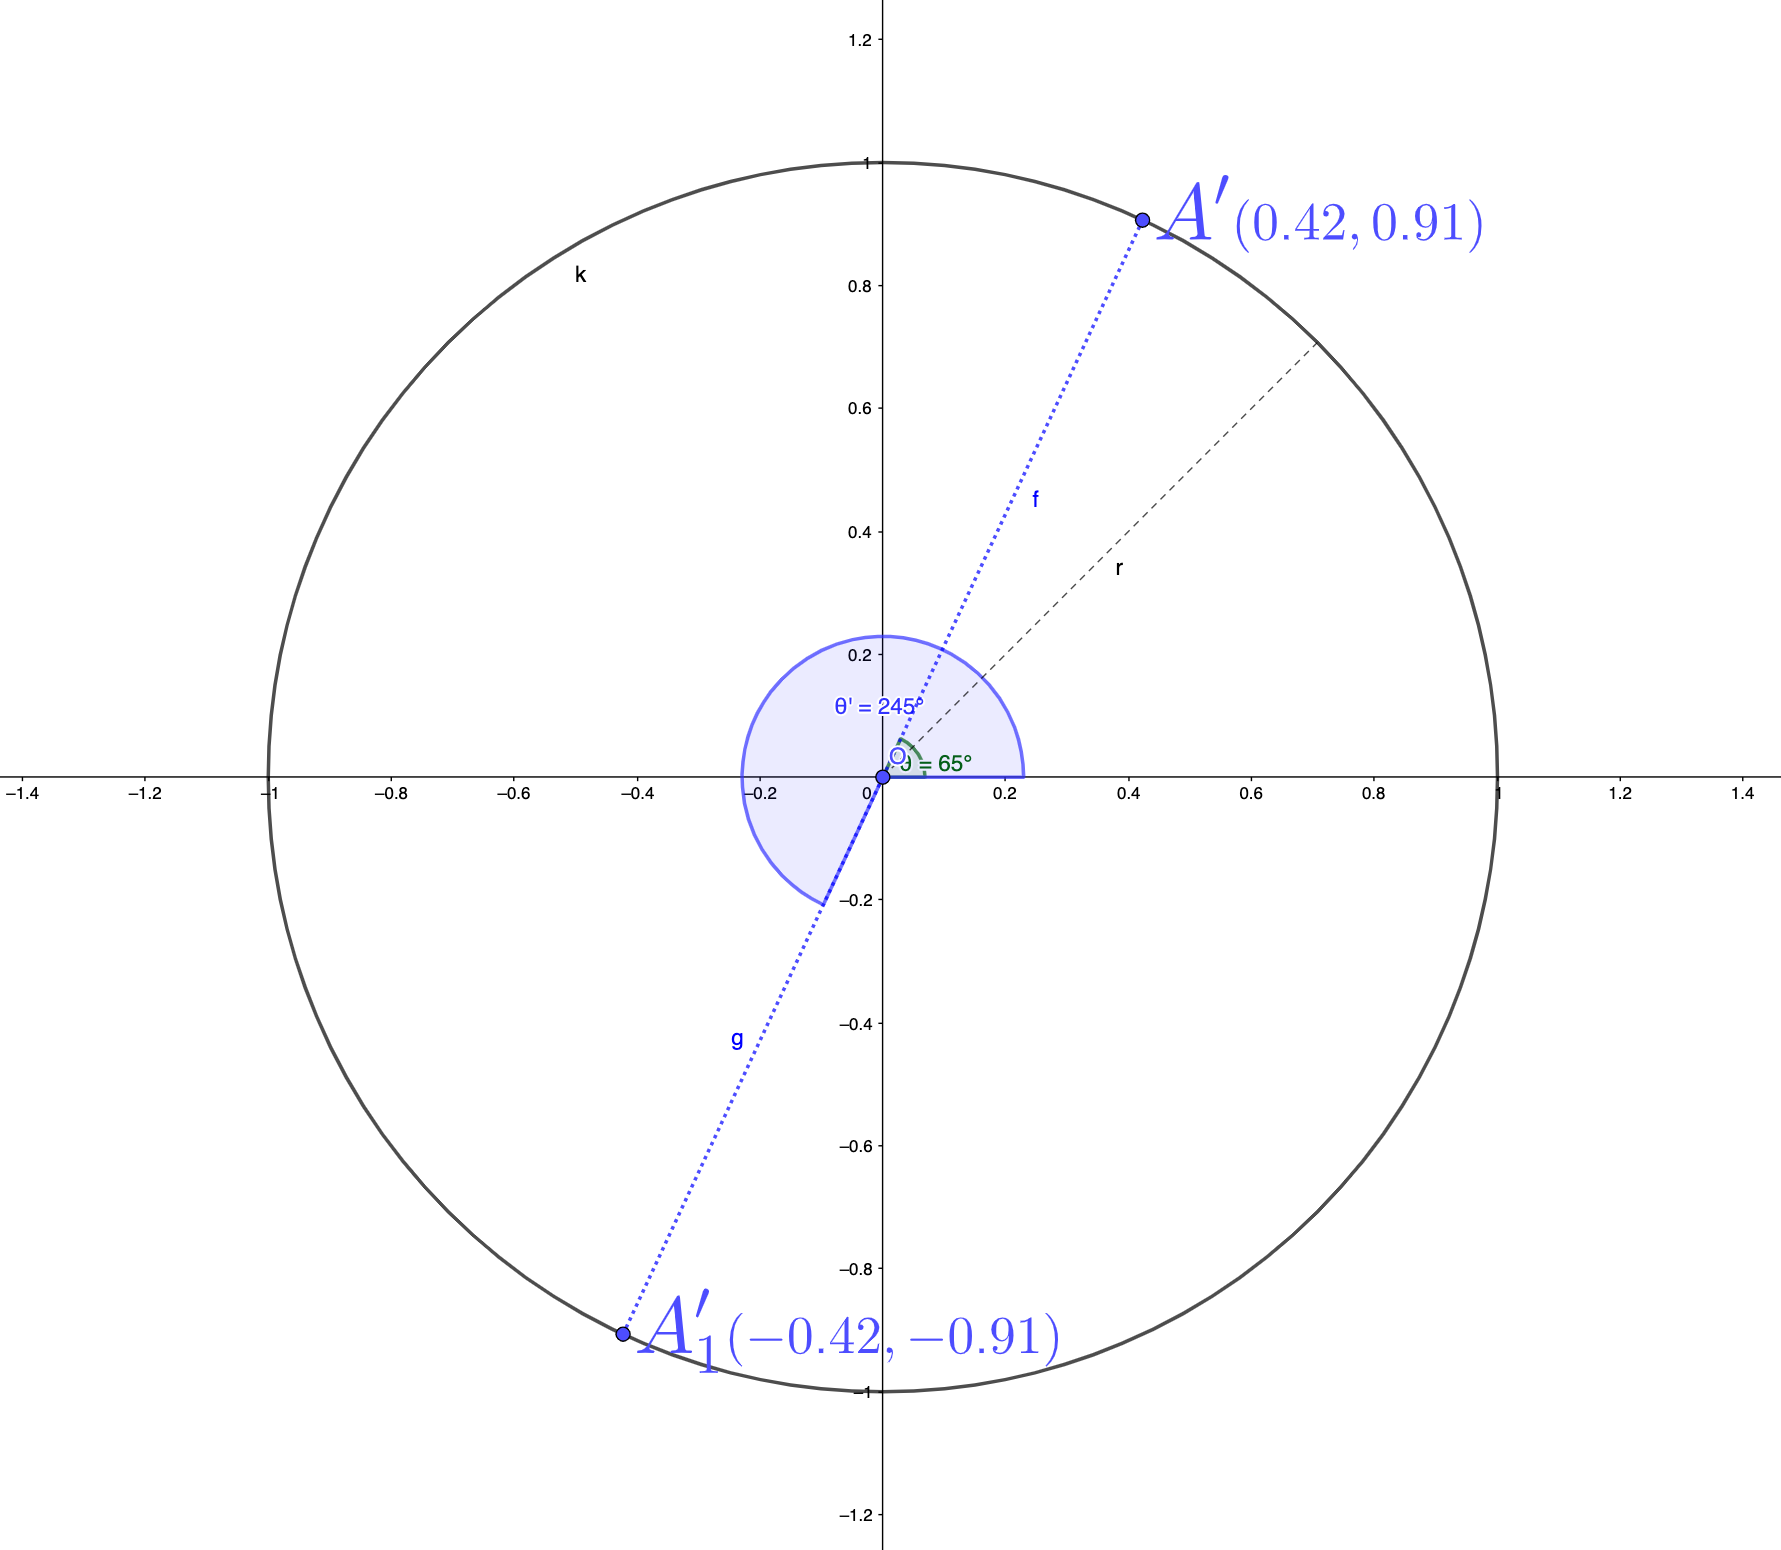
\includegraphics[scale=2.5]{unit_circle_tangent_proof.png}
        \vspace{-10pt}
        \caption{Periodicity of tangent}
        \vspace{-10pt}
    \end{figure}
    
    \textbf{Explanation}: The $period$ of $f:y=sin(x)$ and $f:y=cos(x)$ is $2\pi$, any $x \in D_f$ shifted by the period of $\pi$ will produce a \textbf{function value} for which is valid: $\forall x \in D_f \subset \mathbb{R}: f(x + \pi)=-f(x)$.
    
    Let $A'$ be a point shifted along the circumference $k$ by an angle $\theta$, $A'_1$ be a point shifted along the same circumference by an angle $\theta + \pi$. Their coordinates are depicted using a \textbf{unit circle} and are symmetrical through $O[0,0]$ (point symmetry). Notice: 
    \[
    A'_x = -A'_{x_1} \land A'_y = -A'_{y_1} 
    \]
    
    \textit{Note: an applet is available (\href{https://www.geogebra.org/m/qr7hjqs6}{link}) or scan its \textbf{QR code} under \textbf{Resources}}.
    
    \textbf{Conclusion}
    Function \textbf{tangent} is \textbf{periodic} with the smallest possible
    period $\pi$.
    
    % Parity of tangent
    \item \textbf{Parity}
    \[
    f^+(x):y=tan(x)
    \]
    \[
    f^-(-x):y=tan(-x) = \frac{sin(-x)}{cos(-x)} = \frac{-sin(x)}{cos(x)} = -\frac{sin(x)}{cos(x)} = -tan(x),
    \]
    Based on the parity of \textbf{sine} (odd), \textbf{cosine} (even) $\Rightarrow sin(-x)=-sin(x) \land cos(-x) = cos(x)$.
    
    $f(-x) = -f(x) \Rightarrow$ Tangent is an \textbf{odd function}.
    
    % Monotonicity of tangent
    \item \textbf{Monotonicity}
    
    The tangent function is \textbf{increasing} on $\mathbb{R}$ between 2 consecutive vertical \textbf{asymptotes}, where every asymptote is defined as: $x=(2k + 1)\frac{\pi}{2}, k \in\mathbb{Z}$,\\that is:
    \[
    \forall x_{1,2}\in D_f:tan(x_1)<tan(x_2) \land x_1<x_2 
    \]
    
    \begin{figure}[ht!]
        \centering
        \vspace{-10pt}
        \centering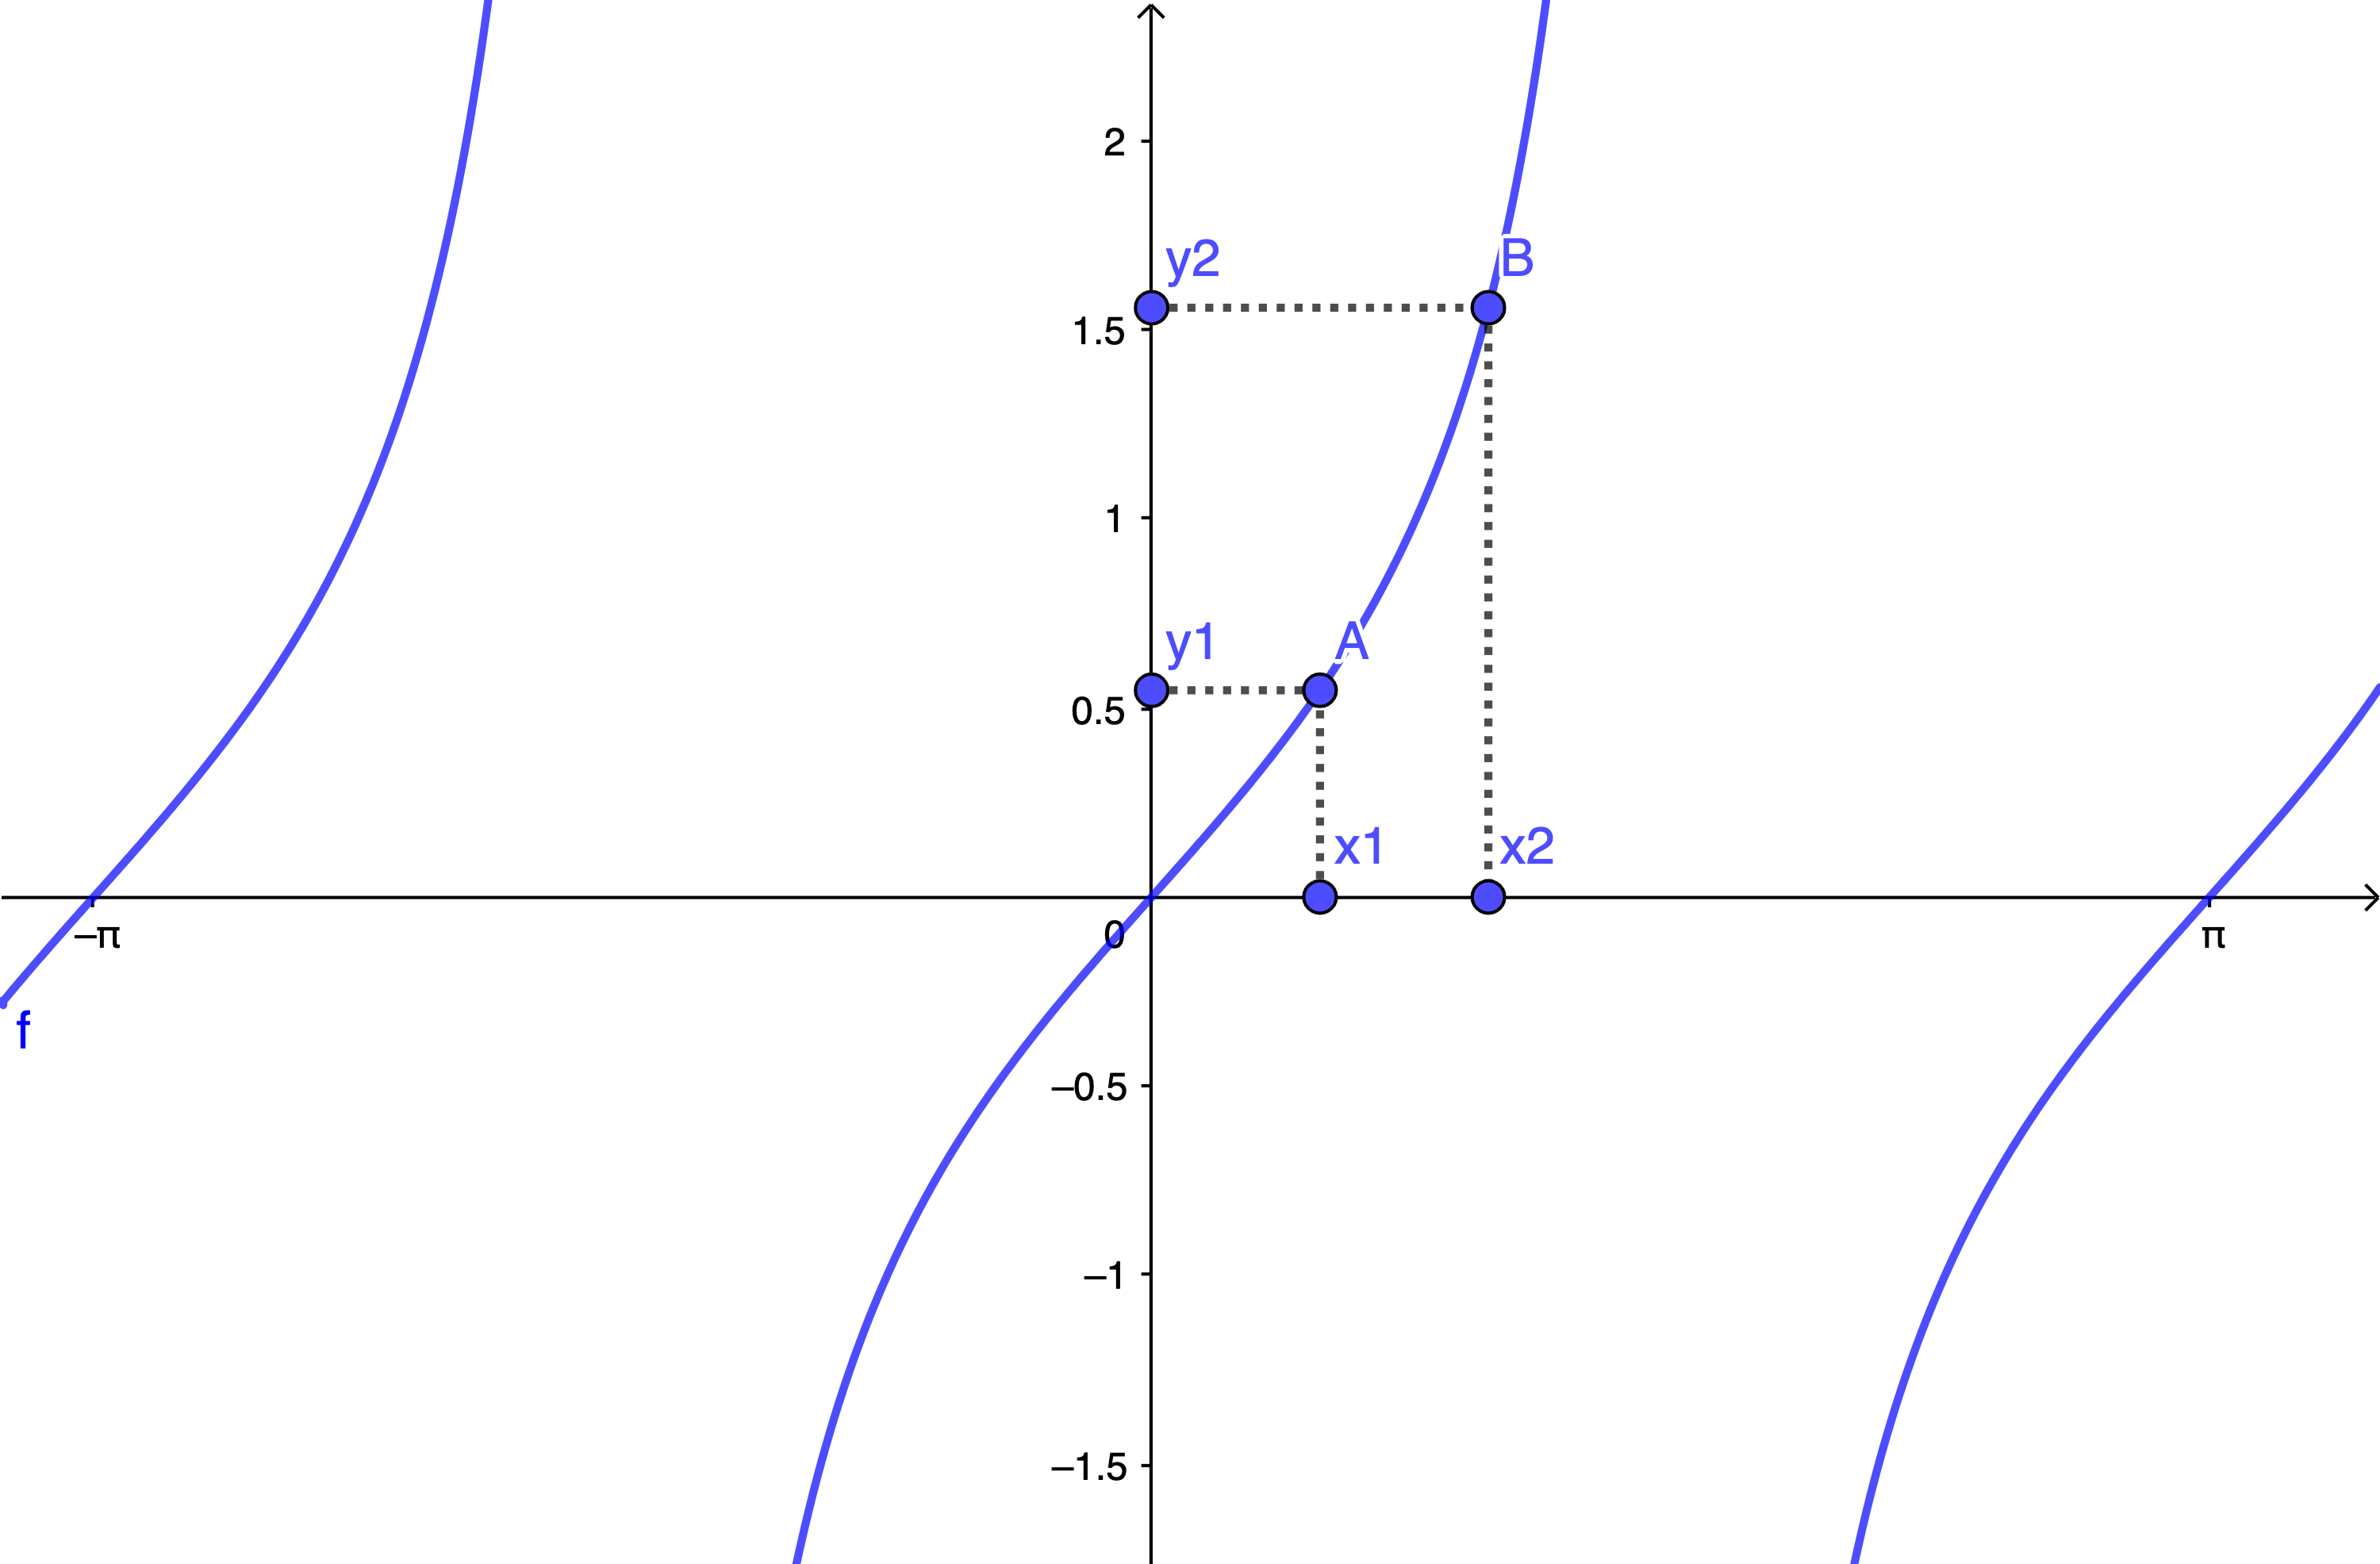
\includegraphics[scale=0.92]{monotony.png}
        \vspace{-10pt}
        \caption{Monotonicity of tangent}
        \vspace{-10pt}
    \end{figure}
    
    \item \textbf{Graph}
    
    \textbf{Tangentoid} is the plot of the tangent function.
    
    \item \textbf{Important function values of tangent}
    
    \begin{center}
    \begin{tabular}{||c c c c c c||} 
    \hline
     $x: $ & $0\degree$ & $30\degree$ & $45\degree$ & $60\degree$ & $90\degree$ \\ [0.5ex] 
     \hline
     $tan(x): $ & 0 & $\frac{\sqrt{3}}{3}$ & 1 & $\sqrt{3}$ & $\text{\O}$ \\ [1ex] 
     \hline
    \end{tabular}
    
    \end{center}
    
\end{enumerate}

% Include scanable resources
\section{\textbf{Resources}}

\centering
\includegraphics[scale=0.05]{applet1.png}

\includegraphics[scale=0.05]{applet2.png}

\centering\textit{Applet 1, Applet 2}

% Plot list of figures
\listoffigures

\end{document}

